\section{Panoramica del Sistema API}

\subsection{Architettura Generale}
L'architettura generale dell'applicazione segue il seguente schema:

\begin{figure}[H]
    \centering
    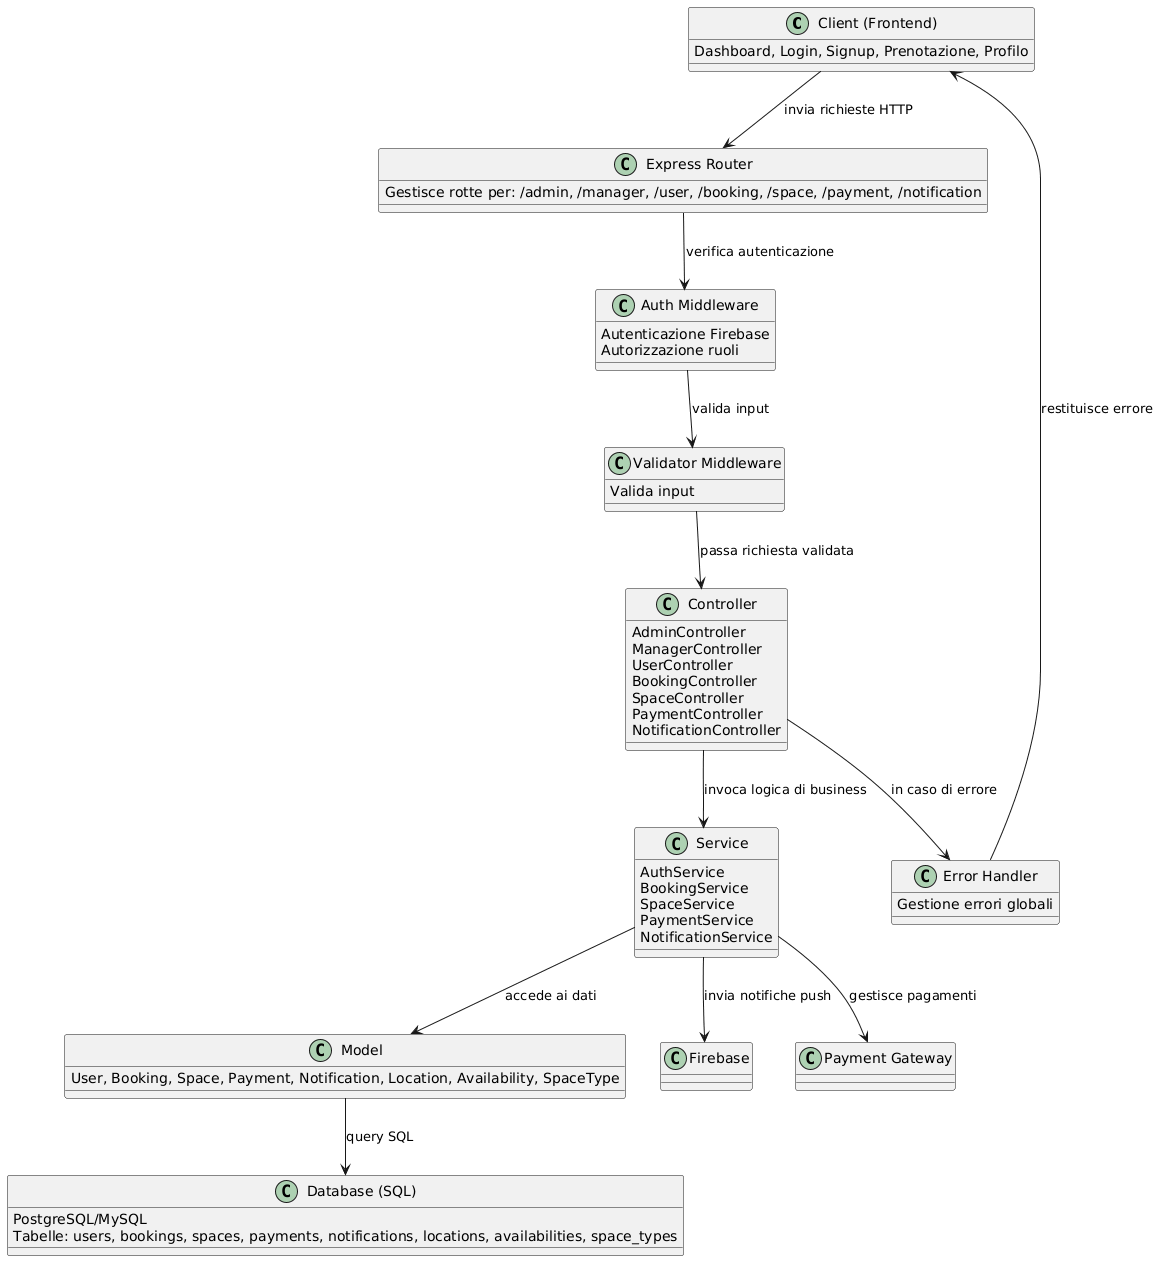
\includegraphics[width=0.8\textwidth]{sections/Schema_architetturale.png}
    \caption{Architettura Generale del Sistema CoWorkSpace}
\end{figure}

\subsection{Architettura REST}
L'API CoWorkSpace implementa un'architettura REST (Representational State Transfer) che segue i principi di design moderni per sistemi distribuiti. Le caratteristiche principali includono:

\begin{itemize}
    \item \textbf{Stateless}: Ogni richiesta è indipendente e contiene tutte le informazioni necessarie
    \item \textbf{Resource-oriented}: Gli endpoint sono organizzati attorno alle risorse del sistema
    \item \textbf{HTTP Methods}: Utilizzo appropriato dei verbi HTTP (GET, POST, PUT, DELETE)
    \item \textbf{JSON Format}: Tutti i dati sono scambiati in formato JSON
    \item \textbf{Consistent Response}: Struttura uniforme delle risposte API
\end{itemize}

\subsection{URL Base e Versioning}
\begin{lstlisting}[style=httpstyle, caption=URL Base dell'API]
# Development
https://localhost:3000/api

# Production
https://api.coworkspace.com/api
\end{lstlisting}

L'API utilizza un approccio basato su path per l'organizzazione degli endpoint senza versioning esplicito nell'URL, seguendo il principio di evoluzione backward-compatible.

\subsection{Formato delle Risposte}
Tutte le risposte dell'API seguono una struttura uniforme per garantire consistenza e facilità di parsing:

\subsubsection{Risposta di Successo}
\begin{lstlisting}[caption=Struttura Risposta di Successo]
{
  "success": true,
  "message": "Operazione completata con successo",
  "data": {
    // Contenuto specifico della risposta
  }
}
\end{lstlisting}

\subsubsection{Risposta di Errore}
\begin{lstlisting}[caption=Struttura Risposta di Errore]
{
  "success": false,
  "message": "Descrizione dell'errore per l'utente",
  "error": "Dettagli tecnici dell'errore",
  "errors": [
    {
      "field": "email",
      "message": "Email non valida"
    }
  ]
}
\end{lstlisting}

\subsection{Codici di Stato HTTP}
L'API utilizza i codici di stato HTTP standard per comunicare l'esito delle operazioni:

\begin{table}[H]
\centering
\begin{tabular}{@{}lp{4cm}p{7cm}@{}}
\toprule
\textbf{Codice} & \textbf{Significato} & \textbf{Utilizzo nell'API} \\
\midrule
\textbf{2xx - Successo} & & \\
200 & OK & Operazione completata con successo \\
201 & Created & Risorsa creata (registrazione, prenotazione) \\
202 & Accepted & Richiesta accettata ma in elaborazione \\
204 & No Content & Operazione completata senza contenuto \\
\midrule
\textbf{4xx - Errori Client} & & \\
400 & Bad Request & Dati di input non validi \\
401 & Unauthorized & Mancanza di autenticazione \\
403 & Forbidden & Mancanza di autorizzazione \\
404 & Not Found & Risorsa non trovata \\
409 & Conflict & Conflitto con stato corrente (email già esistente) \\
422 & Unprocessable Entity & Validazione business logic fallita \\
429 & Too Many Requests & Rate limiting superato \\
\midrule
\textbf{5xx - Errori Server} & & \\
500 & Internal Server Error & Errore interno del server \\
503 & Service Unavailable & Servizio temporaneamente non disponibile \\
\bottomrule
\end{tabular}
\caption{Codici di Stato HTTP Utilizzati}
\end{table}

\subsection{Rate Limiting}
Il sistema implementa rate limiting per proteggere l'API da abusi e garantire qualità del servizio:

\begin{table}[H]
\centering
\begin{tabular}{@{}lll@{}}
\toprule
\textbf{Endpoint} & \textbf{Limite} & \textbf{Finestra Temporale} \\
\midrule
Authentication & 5 tentativi & 15 minuti \\
Password Reset & 5 tentativi & 15 minuti \\
\bottomrule
\end{tabular}
\caption{Configurazione Rate Limiting}
\end{table}

Quando il limite viene superato, l'API restituisce un codice 429 con header informativi:
\begin{lstlisting}[style=httpstyle, caption=Response Headers Rate Limiting]
HTTP/1.1 429 Too Many Requests
X-RateLimit-Limit: 5
X-RateLimit-Remaining: 0
X-RateLimit-Reset: 1640995200
Retry-After: 900

{
  "success": false,
  "message": "Troppi tentativi. Riprova tra 15 minuti."
}
\end{lstlisting}

\subsection{CORS e Sicurezza}
L'API implementa politiche CORS (Cross-Origin Resource Sharing) differenziate per ambiente:

\subsubsection{Sviluppo}
\begin{itemize}
    \item Origini permesse: \texttt{localhost:3000}, \texttt{127.0.0.1:5500}
    \item Metodi: GET, POST, PUT, DELETE, PATCH
    \item Headers: Content-Type, Authorization
    \item Credentials: Supportate
\end{itemize}

\subsubsection{Produzione}
\begin{itemize}
    \item Origini: Solo quelle specificate in \texttt{FRONTEND\_URL}
    \item Politiche più restrittive per sicurezza
    \item Helmet.js per header di sicurezza
\end{itemize}

\subsection{Middleware di Sicurezza}
Il sistema utilizza diversi middleware per garantire la sicurezza:

\begin{table}[H]
\centering
\begin{tabular}{@{}lp{10cm}@{}}
\toprule
\textbf{Middleware} & \textbf{Funzione} \\
\midrule
Helmet & Content Security Policy, prevenzione attacchi XSS \\
CORS & Controllo accessi cross-origin \\
Rate Limiting & Prevenzione attacchi DoS e brute force \\
Input Validation & Validazione e sanitizzazione input utente \\
JWT Authentication & Verifica token di autenticazione \\
Role-based Authorization & Controllo permessi basato sui ruoli \\
\bottomrule
\end{tabular}
\caption{Middleware di Sicurezza Implementati}
\end{table}

\subsection{Gestione degli Errori}
Il sistema implementa una gestione degli errori centralizzata con logging strutturato:

\begin{lstlisting}[caption=Esempio Gestione Errore di Validazione]
{
  "success": false,
  "message": "Dati non validi",
  "errors": [
    {
      "type": "field",
      "field": "email",
      "message": "Email deve essere un indirizzo valido",
      "value": "email-non-valida"
    },
    {
      "type": "field", 
      "field": "password",
      "message": "Password deve contenere almeno 8 caratteri",
      "value": "***"
    }
  ]
}
\end{lstlisting}

\subsection{Gestione Transazioni e Rollback}
Il sistema implementa transazioni database per garantire l'integrità dei dati nelle operazioni complesse:

\subsubsection{Operazioni Transazionali}
Le seguenti operazioni utilizzano transazioni atomiche:

\begin{itemize}
\item \textbf{Elaborazione Pagamenti}: Creazione pagamento + aggiornamento stato prenotazione
\item \textbf{Gestione Disponibilità}: Aggiornamento multiplo slot temporali
\item \textbf{Operazioni SpaceType}: Modifica tipi spazio con validazioni incrociate
\item \textbf{Prenotazioni Complesse}: Creazione prenotazione + blocco disponibilità + notifiche
\end{itemize}

\subsubsection{Pattern di Implementazione}
\begin{lstlisting}[caption=Esempio Transazione Automatica]
// Utility function per transazioni
const transaction = async (callback) => {
  const client = await pool.connect();
  try {
    await client.query('BEGIN');
    const result = await callback(client);
    await client.query('COMMIT');
    return result;
  } catch (error) {
    await client.query('ROLLBACK');
    throw error;
  } finally {
    client.release();
  }
};
\end{lstlisting}

\subsubsection{Strategie di Rollback}
\begin{itemize}
\item \textbf{Rollback Automatico}: In caso di errore, tutte le operazioni della transazione vengono annullate
\item \textbf{Gestione Connessioni}: Rilascio automatico delle connessioni database
\item \textbf{Error Propagation}: Gli errori vengono propagati al livello superiore per logging
\item \textbf{Stato Consistente}: Il database rimane sempre in uno stato coerente
\end{itemize}

\subsubsection{Esempio Pratico: Pagamento con Aggiornamento Prenotazione}
\begin{lstlisting}[caption=Transazione Pagamento Completa]
try {
  await client.query('BEGIN');
  
  // 1. Crea il pagamento
  const payment = await Payment.create({
    booking_id, amount, payment_method, 
    status: 'completed', transaction_id
  });
  
  // 2. Aggiorna stato prenotazione
  await Booking.update(booking_id, { status: 'confirmed' });
  
  await client.query('COMMIT');
  return payment;
} catch (error) {
  await client.query('ROLLBACK');
  throw error;
}
\end{lstlisting}

\newpage

\subsection{Paginazione}
Per gli endpoint che restituiscono liste di dati, l'API supporta paginazione basata su offset:

\begin{lstlisting}[style=httpstyle, caption=Parametri di Paginazione]
GET /api/bookings?page=2&limit=10&sort=created_at&order=desc
\end{lstlisting}

\begin{lstlisting}[caption=Risposta con Metadati di Paginazione]
{
  "success": true,
  "data": {
    "items": [...],
    "pagination": {
      "page": 2,
      "limit": 10,
      "total": 150,
      "totalPages": 15,
      "hasNext": true,
      "hasPrev": true
    }
  }
}
\end{lstlisting}

\subsection{Content-Type e Accept Headers}
L'API supporta esclusivamente JSON per input e output:

\begin{lstlisting}[style=httpstyle, caption=Headers Richiesti]
Content-Type: application/json
Accept: application/json
\end{lstlisting}

\subsection{Documentazione Interattiva}
L'API include documentazione Swagger/OpenAPI accessibile durante lo sviluppo:

\begin{itemize}
    \item \textbf{URL Sviluppo}: \texttt{http://localhost:3000/api-docs}
    \item \textbf{Formato}: OpenAPI 3.0.0
    \item \textbf{Caratteristiche}: Test interattivi, schemi completi, esempi
\end{itemize}

\subsection{Health Check e Monitoring}
Il sistema include endpoint per monitoraggio dello stato:

\begin{lstlisting}[style=httpstyle, caption=Health Check Endpoint]
GET /api/health
\end{lstlisting}

\begin{lstlisting}[caption=Risposta Health Check]
{
  "success": true,
  "data": {
    "status": "ok",
    "timestamp": "2024-01-15T10:30:00Z",
    "version": "1.0.0",
    "database": "connected",
    "uptime": 3600
  }
}
\end{lstlisting}